\section{Design}

\subsection{Overall Architecture}

\subsubsection{Hybrid Solver Architecture Design}

The enhanced SAT solver employs a hybrid architecture that combines proven DPLL algorithmic foundations with graph-aware optimizations, representing a strategic design decision to balance algorithmic sophistication against implementation complexity for moderate-scale graph coloring problems. Rather than implementing a full Conflict-Driven Clause Learning (CDCL) engine with advanced features such as dynamic restart strategies, sophisticated clause deletion policies, and complex implication graph analysis, the design prioritises the integration of domain-specific graph structural knowledge into a reliable solving framework.

This architectural approach addresses the fundamental design challenge that full CDCL implementations, while theoretically superior for large-scale industrial SAT instances, introduce significant implementation complexity that may not provide proportional benefits for the target problem scale of 50-100 vertices. The hybrid design leverages the robustness and simplicity of the existing DPLL solver whilst introducing targeted enhancements that exploit graph colouring problem structure through centrality-based variable ordering and preprocessing optimisations.

The component hierarchy follows a clear separation of concerns: the \texttt{Graph\-Structure\-Analyzer} component computes vertex centrality measures and graph properties, the \texttt{GraphAwarePreprocessor} applies problem-specific optimisations and reductions, and the \texttt{EnhancedCDCLSolver} integrates these insights into the core solving process. This modular architecture enables independent development, testing, and optimisation of each component whilst maintaining clean interfaces and minimising coupling between graph analysis and SAT solving logic.

\begin{figure}[htbp]
\centering
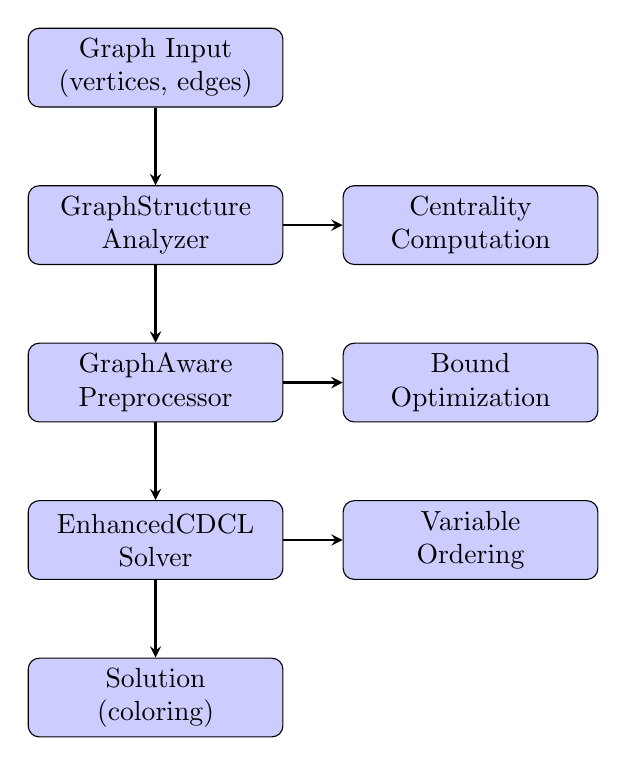
\begin{tikzpicture}[node distance=2cm, auto]
    % Define styles
    \tikzstyle{component} = [rectangle, draw, fill=blue!20, text width=3cm, text centered, rounded corners, minimum height=1cm]
    \tikzstyle{arrow} = [thick,->,>=stealth]
    
    % Main flow components
    \node [component] (input) {Graph Input\\(vertices, edges)};
    \node [component, below of=input] (analyzer) {GraphStructure\\Analyzer};
    \node [component, below of=analyzer] (preprocessor) {GraphAware\\Preprocessor};
    \node [component, below of=preprocessor] (solver) {EnhancedCDCL\\Solver};
    \node [component, below of=solver] (output) {Solution\\(coloring)};
    
    % Main flow arrows
    \draw [arrow] (input) -- (analyzer);
    \draw [arrow] (analyzer) -- (preprocessor);
    \draw [arrow] (preprocessor) -- (solver);
    \draw [arrow] (solver) -- (output);
    
    % Side components showing internal processes
    \node [component, right of=analyzer, xshift=2cm] (centrality) {Centrality\\Computation};
    \node [component, right of=preprocessor, xshift=2cm] (bounds) {Bound\\Optimization};
    \node [component, right of=solver, xshift=2cm] (heuristics) {Variable\\Ordering};
    
    % Side arrows
    \draw [arrow] (analyzer) -- (centrality);
    \draw [arrow] (preprocessor) -- (bounds);
    \draw [arrow] (solver) -- (heuristics);
\end{tikzpicture}
\caption{Enhanced SAT Solver Architecture Overview}
\label{fig:architecture}
\end{figure}


\subsubsection{System Integration Design}

As illustrated in Figure~\ref{fig:integration}, the system integration design prioritises backward compatibility with the existing DPLL solver infrastructure, ensuring that the enhanced solver can function as a drop-in replacement whilst providing additional graph-aware capabilities. The design principle of graceful enhancement means that all existing DPLL functionality remains unchanged and accessible, with graph-aware features providing supplementary optimisation rather than fundamental algorithmic replacement.

Interface design emphasises clean separation between graph analysis and SAT solving concerns through well-defined method signatures and data structures, as depicted in the modular component structure of Figure~\ref{fig:integration}. The fallback strategy ensures robust operation through multiple degradation levels: when graph awareness is disabled, the solver operates identically to the baseline DPLL implementation; when graph analysis fails or produces invalid results, the system defaults to standard variable ordering heuristics; when preprocessing encounters errors, the solver continues with the original problem formulation.

\begin{figure}[htbp]
\centering
\begin{tikzpicture}[node distance=2cm, auto]
    \tikzstyle{component} = [rectangle, draw, fill=blue!20, text width=2.5cm, text centered, rounded corners, minimum height=1cm]
    \tikzstyle{fallback} = [rectangle, draw, fill=red!20, text width=2.5cm, text centered, rounded corners, minimum height=1cm]
    \tikzstyle{decision} = [diamond, draw, fill=yellow!20, text width=2cm, text centered, minimum height=1cm]
    \tikzstyle{arrow} = [thick,->,>=stealth]
    
    \node [component] (input) {Graph Input};
    \node [decision, below of=input] (enabled) {Graph\\Awareness\\Enabled?};
    \node [component, left of=enabled, xshift=-3cm] (baseline) {Baseline DPLL\\Solver};
    \node [component, right of=enabled, xshift=3cm] (enhanced) {Enhanced\\Processing};
    \node [decision, below of=enhanced] (analysis) {Analysis\\Successful?};
    \node [fallback, left of=analysis, xshift=-2cm] (fallback1) {Standard\\Variable\\Ordering};
    \node [component, below of=analysis] (solve) {SAT Solving};
    \node [component, below of=solve] (output) {Solution};
    
    \draw [arrow] (input) -- (enabled);
    \draw [arrow] (enabled) -- node {No} (baseline);
    \draw [arrow] (enabled) -- node {Yes} (enhanced);
    \draw [arrow] (enhanced) -- (analysis);
    \draw [arrow] (analysis) -- node {No} (fallback1);
    \draw [arrow] (analysis) -- node {Yes} (solve);
    \draw [arrow] (fallback1) -- (solve);
    \draw [arrow] (baseline) |- (output);
    \draw [arrow] (solve) -- (output);
\end{tikzpicture}
\caption{System Integration with Fallback Mechanisms}
\label{fig:integration}
\end{figure}

\subsubsection{Scalability Design Considerations}

The architecture explicitly targets moderate-scale graph colouring problems in the 50-100 vertex range through adaptive complexity management that balances preprocessing investment against search space reduction benefits. For smaller problems below 50 vertices, the design employs comprehensive graph analysis including betweenness centrality computation, whilst larger instances utilise faster degree-based centrality measures to maintain reasonable preprocessing overhead.

Complexity management decisions prioritise $O(V+E)$ preprocessing algorithms over $O(V^3)$ advanced analysis techniques based on the observation that preprocessing time must remain small relative to expected solving time for the target problem scale. The performance trade-off design acknowledges that preprocessing investment should scale appropriately with problem difficulty.

\subsection{SAT Solver Core Design}

\subsubsection{Variable Ordering Heuristic Design}

The core innovation of the enhanced solver lies in its variable ordering heuristic design, which replaces traditional frequency-based or random variable selection with graph centrality-driven prioritisation. The implementation utilizes an adaptive weighting strategy that adjusts centrality measure importance based on graph structural characteristics.

For sparse graphs (density < 0.3), degree centrality receives 70\% weight while betweenness centrality receives 30\% weight, reflecting that high-degree vertices create significant constraint bottlenecks in sparsely connected structures. Dense graphs (density > 0.7) employ inverse weighting with degree centrality at 40\% and betweenness centrality at 60\%, recognizing that betweenness better identifies critical structural positions when most vertices have similar high degrees. Medium density graphs (0.3 ≤ density ≤ 0.7) utilize balanced weighting of 60\% degree centrality and 40\% betweenness centrality.

% INSERT THE ADAPTIVE WEIGHTING FIGURE HERE
\begin{figure}[htbp]
\centering
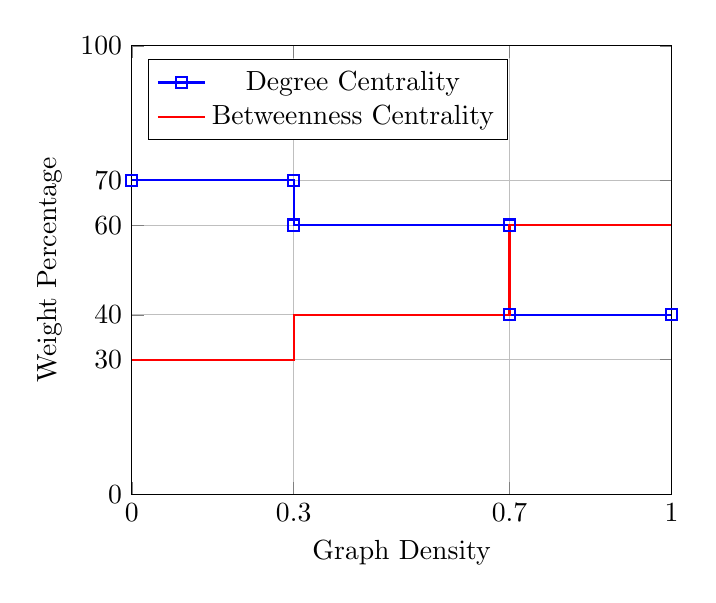
\begin{tikzpicture}
    \begin{axis}[
        xlabel={Graph Density},
        ylabel={Weight Percentage},
        xmin=0, xmax=1,
        ymin=0, ymax=100,
        xtick={0, 0.3, 0.7, 1},
        ytick={0, 30, 40, 60, 70, 100},
        legend pos=north west,
        grid=major
    ]
    
    \addplot[blue, thick, mark=square] coordinates {
        (0, 70) (0.3, 70) (0.3, 60) (0.7, 60) (0.7, 40) (1, 40)
    };
    
    \addplot[red, thick, mark=circle] coordinates {
        (0, 30) (0.3, 30) (0.3, 40) (0.7, 40) (0.7, 60) (1, 60)
    };
    
    \legend{Degree Centrality, Betweenness Centrality}
    \end{axis}
\end{tikzpicture}
\caption{Adaptive Centrality Weighting Based on Graph Density}
\label{fig:adaptive-weighting}
\end{figure}

The final variable priority computation integrates three components through weighted combination: graph structure influence (50\%), symmetry breaking influence (20\%), and learning-based influence (30\%). This creates a composite priority score that balances structural graph properties with SAT solver dynamics.

The implementation design pre-computes a complete variable priority ordering during the preprocessing phase, creating a sorted list that maps SAT variables to their corresponding graph-theoretic importance scores. Caching design optimisations store the computed variable ordering in the \texttt{\_variable\_priority\_order} attribute, eliminating redundant centrality calculations across multiple decision points.

\subsubsection{Enhanced Decision Making Design}

The enhanced decision making design adopts a conservative approach that preserves the reliability of the underlying DPLL algorithm whilst incorporating graph-aware improvements. Rather than implementing complex decision heuristics that might introduce algorithmic instability, the design focuses on improving variable selection quality through structural analysis whilst maintaining standard value assignment strategies.

The branching strategy implementation utilises the priority-ordered variable selection mechanism through the \texttt{\_dpll\_with\_custom\_ordering} method, which recursively applies the enhanced variable ordering whilst preserving traditional true/false value exploration. State management enhancements include comprehensive statistics tracking through the \texttt{enhanced\_stats} dictionary, enabling detailed analysis of solver behaviour and performance characteristics.

\subsubsection{Conflict Resolution Design}

The conflict resolution design deliberately emphasises simplicity and reliability over algorithmic sophistication, reflecting the design philosophy that moderate-scale problems benefit more from improved variable ordering than from complex conflict analysis mechanisms. The implementation leverages the existing DPLL backtracking infrastructure rather than implementing sophisticated clause learning or non-chronological backtracking features.

The design choice to utilise simple backtracking rather than advanced CDCL techniques stems from the observation that the target problem scale rarely requires the memory and learning capabilities that justify CDCL's implementation complexity. Future extensibility considerations ensure that the current architecture can accommodate more sophisticated conflict resolution mechanisms without requiring fundamental restructuring.

\subsection{Graph Coloring Specializations}

\subsubsection{Graph Analysis Design}

The graph analysis design centres on efficient computation and storage of vertex centrality measures that inform SAT variable prioritisation decisions. The \texttt{GraphStructure\-Analyzer} class implements a comprehensive analysis pipeline that constructs adjacency representations, computes multiple centrality measures, and provides efficient access to graph structural properties throughout the solving process.

Centrality computation design employs degree centrality as the primary measure due to its $O(V+E)$ computational complexity and direct relevance to constraint density in graph colouring problems. Data structure design utilises adjacency list representation through the \texttt{adjacency} dictionary, providing efficient neighbour enumeration for centrality calculations whilst minimising memory overhead.

\subsubsection{Preprocessing Strategy Design}

The preprocessing strategy design implements a multi-stage pipeline that systematically reduces problem complexity through graph-specific optimisations before SAT encoding generation. The \texttt{GraphAwarePreprocessor} class orchestrates this pipeline through the \texttt{preprocess\_graph\_coloring\_instance} method, which applies sequential optimisation steps whilst maintaining problem equivalence.

Problem reduction design addresses common graph colouring simplifications through the \texttt{\_remove\_isolated\_vertices} method, which identifies and eliminates vertices with no incident edges since these can be coloured arbitrarily without affecting solution validity. Bound optimisation design integrates Brooks' theorem through the \texttt{\_optimize\_\-color\_\-bound} method, which computes theoretical upper bounds on chromatic number based on maximum degree analysis.

\subsubsection{Symmetry Breaking Design}

The symmetry breaking design targets colour permutation symmetries through lexicographic ordering constraints that eliminate equivalent solutions differing only in colour label assignment. The approach design focuses exclusively on colour symmetries rather than attempting to address vertex symmetries, which require more complex automorphism detection and constraint generation.

Implementation design generates symmetry breaking clauses through the \texttt{\_generate\_\-symmetry\_\-breaking\_\-clauses} method, which creates lexicographic ordering constraints ensuring that colour indices are used in ascending order. Integration design treats symmetry breaking as an additive enhancement to existing CNF encodings rather than a fundamental modification, ensuring compatibility with various encoding strategies whilst providing consistent symmetry reduction benefits.